% Beamer presentation
\documentclass[11pt,aspectratio=43,ignorenonframetext,t]{beamer}

% Presentation settings
\mode<presentation>{
  \usetheme[framenumber,titleframestart=1]{UoM_alex}
  \usefonttheme{professionalfonts} % using non standard fonts for beamer
  \usefonttheme{serif}
  \usepackage{fontspec}
  \setmainfont[Ligatures=TeX]{Arial}
}

% Handout settings
\mode<article>{
  \usepackage{fullpage}
  \usepackage{fontspec}
  \setmainfont[Ligatures=TeX]{Arial}
  \setlength{\parskip}{1.5\baselineskip} % correct beamer line spacings
  \setlength{\parindent}{0cm}
  \usepackage{enumitem}
  \setlist[itemize]{topsep=0pt}
}

 % Packages
\usepackage{graphicx}
\graphicspath{{./images/png}} % generic graphics path; overridden if necessary
\usepackage{amsmath}
\allowdisplaybreaks[1] % allow eqnarrays to break across pages
\usepackage{amssymb} 
\usepackage[HTML]{xcolor}
\definecolor{uomlinkblue}{HTML}{0071BC}
\usepackage{hyperref}
\hypersetup{
  colorlinks=true,
  linkcolor=uomlinkblue,
  filecolor=uomlinkblue,      
  urlcolor=uomlinkblue,
  pdflang={en-GB},
}
\usepackage[document]{ragged2e} % left aligned text for accessibility
\usepackage{tikz}
\usetikzlibrary{positioning, arrows, arrows.meta}
\usepackage{unicode-math} % unicode maths for accessibility
\usepackage{pdfcomment}   % for alt text for accessibility
\usepackage{rotating}     % allow portrait figures and tables
\usepackage{subfigure}    % allow matrices of figures
\usepackage{float}        % allows H option on floats to force here placement
\usepackage{multirow}     % allows merging of rows in tables
\usepackage{tabularx}     % allows fixed width tables
\usepackage{ctable}       % modifies \hline for use in table
\usepackage{bm}           % allow bold fonts in equations
\usepackage{pgf}          % allow graphics manipulation
\usepackage{etoolbox}
  
% Custom commands
\newcolumntype{Z}{>{\centering\arraybackslash}X}  % tabularx centered columns 

\makeatletter
  \DeclareRobustCommand{\em}
  {
    \@nomath\em
    \if b
      \expandafter\@car\f@series\@nil \normalfont
    \else
      \bfseries
    \fi
  }
\makeatother

\makeatletter
  \preto{\@verbatim}{\topsep=0pt \partopsep=0pt}
\makeatother

\def\checkmark{
  \tikz\fill[scale=0.4](0,.35) -- (.25,0) -- (1,.7) -- (.25,.15) -- cycle;
}

% Counters
\newcounter{example_number} % keep track of the example questions

% Frontmatter
\newcommand{\cmclecture}[1]{
  \title{Combinatorial Mesh Calculus (CMC): Lecture #1}
}
\author{
  Lectured by:
  \href{https://scholar.google.com/citations?user=x4R-snQAAAAJ&hl=en}
  {Dr. Kiprian Berbatov}$^1$\\
  \smallskip
  Lecture Notes Compiled by:
  \href{https://scholar.google.com/citations?user=CoIpITkAAAAJ&hl=en}
  {Muhammad Azeem}$^1$\\
  \smallskip
  Under the supervision of:
  \href{https://scholar.google.co.uk/citations?user=3nWJe5wAAAAJ&hl=en}
  {Prof. Andrey P. Jivkov}$^1$\\
  \smallskip
  {\tiny $^1$Department of Mechanical and Aerospace Engineering,
    The University of Manchester, Oxford Road, Manchester M13 9PL, UK}
}

% Special frames
\newcommand{\cmctitleframe}{
  \titlepage
  \begin{tikzpicture}[remember picture,overlay]
    \node[anchor=south east] at (current page.south east) {
      \href{https://youtube.com/@kipi.berbatov}{
        
\includegraphics[width=1.5cm]{youtube-icon.png}
      }
    };
  \end{tikzpicture}
}
\newcommand{\cmcendframe}{
  \begin{figure}
    \centering
    
\includegraphics[width=0.85\linewidth]{Thanks.png}
  \end{figure}
}

\graphicspath{{./images/png}{./images/png/lecture-01}}
\cmclecture{1}
\date{13 October 2025}

\begin{document}

%========================= TITLE =========================
\begin{frame}
  \cmctitleframe
\end{frame}

\section{Basic Sets and Notation}

\begin{frame}{Basic Definitions}
\begin{itemize}
  \item \textbf{Natural numbers:}
     $\mathbb{N} = \{0,1,2,3,\dots\} \quad\text{or}\quad \{1,2,3,\dots\},$ choice depends on convention.
  \item \textbf{Positive naturals:}  $\mathbb{N}^{+} = \{1,2,3,\dots\}$
  \item \textbf{Integers:} $\mathbb{Z} = \{\dots,-2,-1,0,1,2,\dots\}$
  \item \textbf{Positive integers:}  $\mathbb{Z}^{+} = \{1,2,3,\dots\}$
  \item \textbf{Rational numbers:} $\mathbb{Q} = \left\{ \frac{p}{q} \mid p \in \mathbb{Z},\, q \in \mathbb{Z}\setminus\{0\} \right\}$
  \item \textbf{Positive rationals:} $\mathbb{Q}^{+} = \{q \in \mathbb{Q} \mid q > 0\}$
  \item \textbf{Real numbers:} $\mathbb{R} = \{ x \mid -\infty < x < \infty \}$
  \item \textbf{Positive reals:} $\mathbb{R}^{+} = \{ x \in \mathbb{R} \mid x > 0\}$
\end{itemize}
\end{frame}

\begin{frame}{Basic Definitions}
\begin{figure}
    \centering
    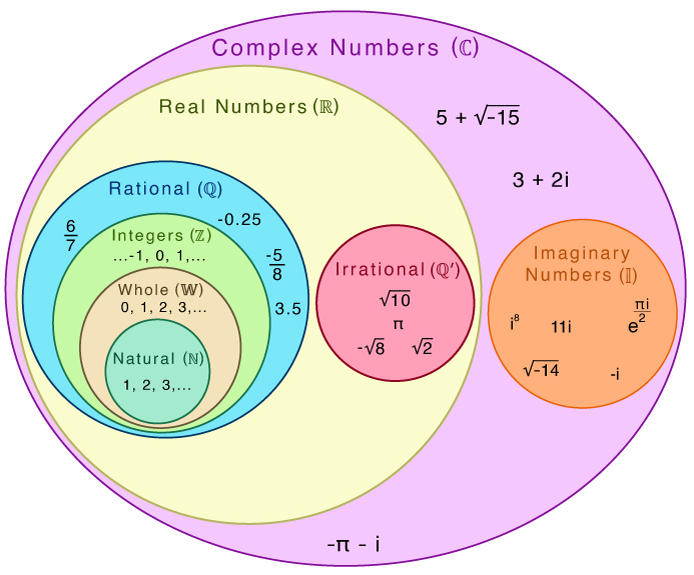
\includegraphics[width=0.7\linewidth]{Number-Sets-Venn-Diagram.png}
\end{figure}

\end{frame}

\begin{frame}{Set-Builder / Predicate Notation}
Let a property $\varphi(x)$ and a set $A$
\begin{align*}
  B = \{\, x \in A \mid \varphi(x) \text{ is true} \}
\end{align*}
means “the subset of \(A\) whose members satisfy property \(\varphi\).”


\begin{block}{Examples:}
\vspace{-0.2cm}

\begin{itemize}
    \item Positive rational numbers can be written like
    $$\mathbb{Q}^{+} = \{ x \in \mathbb{Q} \mid x > 0\}, \qquad
  \mathbb{N} = \{ n \in \mathbb{Z} \mid n \ge 0 \}$$
\item If \(X\) is a set and \(n \in \mathbb{N}\), define
\begin{align*}
  X^n = \{ (x_1, x_2, \dots, x_n) \mid x_i \in X \, \, \,\text{for}\, i = 1,\dots,n\}.
\end{align*}
\item If \(m,n \in \mathbb{N}\), define the set of \(m\times n\) matrices over \(X\):
\begin{align*}
  M_{m \times n}(X) = \left\{\, [a_{ij}] \mid a_{ij} \in X,\; 1 \le i \le m,\,1 \le j \le n\right\}.
\end{align*}
\end{itemize}

\end{block}
\end{frame}

\section{Logic: Connectives and Quantifiers}

\begin{frame}{Logical Connectives: Basic Laws}
Let \(\varphi\) and \(\psi\) be logical statements (predicates). We have:
\begin{block}{}
\hspace{-2cm}
\begin{align*}
\begin{aligned}
\neg (\neg \varphi) &\equiv \varphi &\text{ (negation)}, \\
\varphi \land \psi &\text{ (conjunction/logical AND)}, \\
\varphi \lor \psi &\text{ (disjunction/logical OR)}, \\
\varphi \implies \psi &\text{ (implication)}, \\
\varphi \iff \psi &\text{ (bi-conditional, equivalence)}.
\end{aligned}
\end{align*}
\end{block}

Some equivalences:
\begin{align*}
\varphi \implies \psi \;\equiv\; \neg \varphi \lor \psi, \quad
\neg(\varphi \land \psi) \equiv \neg \varphi \lor \neg \psi \quad (\text{De Morgan}), \dots
\end{align*}
\end{frame}

\begin{frame}{Quantifiers: $\forall$, $\exists$}
  \begin{block}{Universal quantifier:}
  $$\forall x \in A,\; \varphi(x):\!\! \text{ for all } x \text{ in } A, \varphi(x)\text{ holds.}$$
  \end{block}
  \begin{block}{Existential quantifier:}
  $$\exists x \in A,\; \varphi(x) \;:\!\! \text{ there is at least one } x \in A \text{ with } \varphi(x).$$
\end{block}

Negation rules:
\begin{align*}
  \neg \bigl(\forall x \in A\, \varphi(x)\bigr) \;\equiv\; \exists x \in A\, \neg\varphi(x),
\end{align*}
\begin{align*}
  \neg \bigl(\exists x \in A\, \varphi(x)\bigr) \;\equiv\; \forall x \in A\, \neg\varphi(x).
\end{align*}
\end{frame}

\begin{frame}{Continuity and Uniform Continuity}
\begin{block}{Continuity}
Let \(I \subset \mathbb{R}\) be an interval, \(f: I \to \mathbb{R}\). We say \(f\) is continuous if
\begin{align*}
\forall x \in I,\; \forall \varepsilon>0,\; \exists \delta>0,\; \forall y \in I,\;
|x-y|<\delta \implies |f(x) - f(y)| < \varepsilon.
\end{align*}
\end{block}
\begin{block}{Uniform continuity} \(f\) is uniformly continuous if
\begin{align*}
\forall \varepsilon>0,\; \exists \delta>0,\; \forall x,y \in I,\;
|x-y|<\delta \implies |f(x) - f(y)| < \varepsilon.
\end{align*}
\end{block}
\vspace{-0.8cm}
\begin{block}{Remark:}
    Uniform continuity is a stronger (global) condition: \(\delta\) must work for all \(x\), not depend on \(x\).
\end{block}
\end{frame}


\begin{frame}{Sets}
\begin{block}{Let \(A, B\) be sets.}
Then\vspace{-0.5cm}
\begin{align*}
A \cup B = \{ x \mid x\in A \;\text{or}\; x\in B\}, \\
A \cap B = \{ x \mid x\in A \;\text{and}\; x\in B\}, \\
A \setminus B = \{ x \mid x\in A \;\text{and}\; x\notin B\}.
\end{align*}
\end{block}

\begin{block}{Power set:}
Boolean algebra of subsets
\begin{align*}
\mathcal{P}(A) = \{\, S \mid S \subseteq A \,\}\qquad |\mathcal{P}(A)| = 2^{|A|}
\end{align*}

\end{block}
\end{frame}

\begin{frame}{Sets}
\begin{block}{Remarks:}
\begin{itemize}
  \item Each element of $\mathcal{P}(A)$ is a subset of $A$ (including $\emptyset$ and $A$ itself).
  \item If $A$ has $n$ elements, then $\mathcal{P}(A)$ has $2^n$ elements.
  \item Equipped with the operations of union ($\cup$), intersection ($\cap$), and complement ($^c$), $\mathcal{P}(A)$ forms a \textbf{Boolean algebra}.
  \item The smallest element (zero) is $\emptyset$, and the greatest element (unity) is $A$.
\end{itemize}
\end{block}
\end{frame}

\begin{frame}{Visualisation}
\begin{figure}
    \centering
    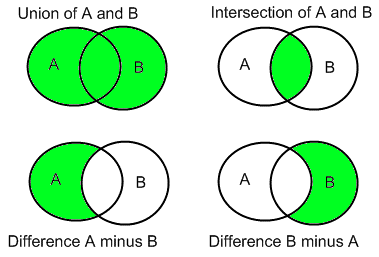
\includegraphics[width=0.7\linewidth]{Image2.png}
\end{figure}
Venn diagrams to illustrate union, intersection, difference.
\end{frame}

\begin{frame}{Visualisation}
\begin{figure}
    \centering
    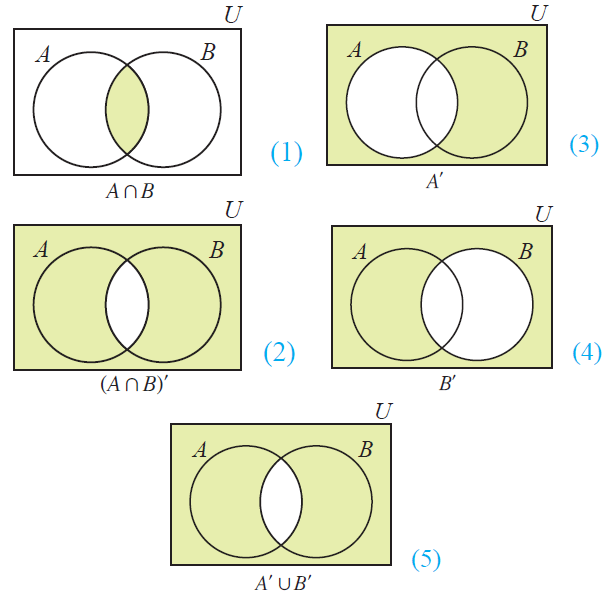
\includegraphics[width=0.7\linewidth]{Image3.png}
\end{figure}
\end{frame}

\begin{frame}{Ordered Pairs and Cartesian Product}
\begin{block}{Definition:} The ordered pair \((a,b)\) is defined by the Kuratowski construction:
\begin{align*}
(a,b) = \{ \{a\}, \{a,b\} \}.
\end{align*}
One checks \((a,b) = (a^{'},b^{'})\) iff \(a=a^{'}\) and \(b=b^{'}\).

\medskip

\textbf{Cartesian product:}
\begin{align*}
A \times B = \{ (a,b) \mid a \in A,\; b \in B \}.
\end{align*}

\medskip

\textbf{Cardinality (finite case):} If \(|A| = m, |B| = n\), then
\begin{align*}
|A \times B| = m \cdot n.
\end{align*}
More generally, for \(X^n\), \(|X^n| = |X|^n\) for finite \(X\).
\end{block}
\end{frame}

\section{Functions and Composition}

\begin{frame}{Function and Equality of Functions}
Let \(X, Y\) be sets. A \emph{function} \(f: X \to Y\) ($X \xrightarrow{f} Y$) is a subset
\begin{align*}
f \subseteq X \times Y
\end{align*}
such that
\begin{itemize}
  \item For every \(x \in X\), there is a unique \(y \in Y\) with \((x,y) \in f\).
\end{itemize}

\medskip
\begin{block}{Definition}
Two functions \(f, g: X \to Y\) are \emph{equal}, \(f = g\), if
\begin{align*}
\forall x \in X,\; f(x) = g(x).
\end{align*}
\end{block}
\vspace{-0.5cm}

\begin{block}{Example:} \(\sin^2 x + \cos^2 x = 1\) defines a function identically equal to constant function \(1(x)=1\), for domain \(\mathbb{R}\).
\end{block}
\end{frame}



\begin{frame}{Composition of Functions}
If \(f: X \to Y\) and \(g: Y \to Z\), define
\begin{align*}
g \circ f: X \to Z, \quad (g \circ f)(x) = g(f(x)).
\end{align*}

\medskip

\textbf{Associativity:} If \(h: Z \to W\), then
\begin{align*}
h \circ (g \circ f) = (h \circ g) \circ f.
\end{align*}
\vspace{-0.5cm}
\begin{block}{Example:}
Let  $X = \{a,b,c\},\; Y = \{0,1\},\; Z = \{w,x,y,z\}.$ Define
\begin{align*}
f(a)=0,\; f(b)=1,\; f(c)=0, \quad
g(0)=w,\; g(1)=z.
\end{align*}
Then \(g \circ f\) maps \(a\mapsto w\), \(b\mapsto z\), \(c\mapsto w\).
You can draw arrow diagrams:
$X \xrightarrow{f} Y \xrightarrow{g} Z$
\end{block}
\end{frame}


\begin{frame}{Visualization}
    \begin{figure}
        \centering
        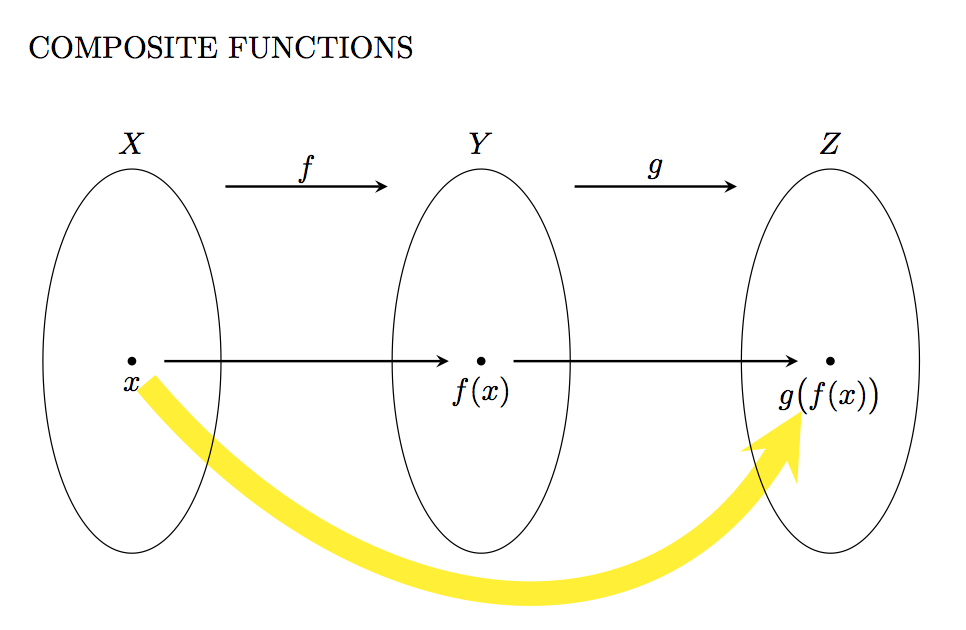
\includegraphics[width=0.8\linewidth]{Image4.png}
    \end{figure}
\end{frame}

\begin{frame}{Axiom of Set Equality:}
\textbf{Axiom (Extensionality).}
Let $X$ and $Y$ be two sets. Then
\[
X = Y \iff \bigl( X \subseteq Y \ \text{and}\  Y \subseteq X \bigr),
\]
that is,
\[
X = Y \iff \bigl( \forall x\, (x \in X \Rightarrow x \in Y) \bigr)
\ \text{and}\
\bigl( \forall x\, (x \in Y \Rightarrow x \in X) \bigr).
\]
\textbf{Interpretation:} Two sets are equal if and only if they contain exactly the same elements.

\begin{exampleblock}{Example: Let $A = \{1,2,3\}$ and $B = \{x \in \mathbb{N} \mid x < 4\}$.}
\textbf{Proof.}
\begin{itemize}
  \item[$(1)$] If $x \in A$, then $x \in \{1,2,3\}$, hence $x < 4$ and $x \in B$. Thus $A \subseteq B$.
  \item[$(2)$] If $x \in B$, then $x < 4$ and $x \in \mathbb{N}$, so $x \in \{1,2,3\}=A$. Hence $B \subseteq A$.
\end{itemize}
By the Axiom of Extensionality, $A=B$.

\textbf{Corollary (Intersection Form):}
If $A \cap C = B \cap C$ for every $C$, then $A=B$ since identical intersections imply identical elements. $\square$
\end{exampleblock}
\end{frame}

\begin{frame}{Identity Function and Its Property}
\vspace{-0.4cm}
\begin{block}{Definition:} For any set \(X\), the identity function is
\begin{align*}
\mathrm{id}_X: X \to X, \quad \mathrm{id}_X(x) = x \quad \forall x \in X.
\end{align*}
\end{block}

\vspace{-0.5cm}
\begin{block}{Proposition:}
For any function \( f: X \to Y \),\\ $f \circ \mathrm{id}_X = f, \qquad \mathrm{id}_Y \circ f = f.$
\end{block}
\vspace{-0.4cm}
\begin{proof}
Let \(x \in X\).
By definition of composition: $
(f \circ \mathrm{id}_X)(x) = f(\mathrm{id}_X(x)) = f(x),$  since \(\mathrm{id}_X(x) = x\).
Hence \(f \circ \mathrm{id}_X = f.\)

Similarly, for the right composition: $(\mathrm{id}_Y \circ f)(x) = \mathrm{id}_Y(f(x)) = f(x),$ since \(\mathrm{id}_Y(y) = y\) for all \(y \in Y\).
Thus \(\mathrm{id}_Y \circ f = f.\) \(\square\)
\end{proof}
\end{frame}

\begin{frame}{Injective, Surjective, Bijective}
Let \(f: X \to Y\).

\begin{itemize}
  \item \(f\) is \textbf{injective} (one-to-one) if
  \begin{align*}
    \forall x_1, x_2 \in X,\; f(x_1) = f(x_2) \implies x_1 = x_2.
  \end{align*}
  \item \(f\) is \textbf{surjective} (onto) if
  \begin{align*}
    \forall y \in Y,\; \exists x \in X,\; f(x) = y.
  \end{align*}
  \item \(f\) is \textbf{bijective} if it is both injective and surjective.
\end{itemize}

\textbf{Examples:}
\begin{itemize}
    \item \(\mathrm{id}_X\) is bijective.
    \item \(f(x) = x^2\) on \(\mathbb{R} \to \mathbb{R}\) is not injective (two preimages);
    \item restrict to \([0,\infty)\), then it becomes injective (and bijective onto \([0,\infty)\)).
\end{itemize}
\end{frame}

\begin{frame}{Left Inverse, Right Inverse, and Relation}
Let \(f: X \to Y\).

\begin{itemize}
  \item A \textbf{left inverse} of \(f\) is a function \(g: Y \to X\) such that
  \begin{align*}
    g \circ f = \mathrm{id}_X.
  \end{align*}
  \item A \textbf{right inverse} of \(f\) is a function \(h: Y \to X\) such that
  \begin{align*}
    f \circ h = \mathrm{id}_Y.
  \end{align*}
  \item If a function has both a left inverse and a right inverse, they coincide and that common map is called the \emph{inverse} \(f^{-1}\).
\end{itemize}


\textbf{Proposition:}
\begin{enumerate}
  \item \(f\) has a left inverse \(\iff\) \(f\) is injective.
  \item \(f\) has a right inverse \(\iff\) \(f\) is surjective.
  \item \(f\) is bijective \(\iff\) \(f\) has a two-sided inverse.
\end{enumerate}

\emph{Proofs:} ???
\end{frame}

\begin{frame}{Proof }
\textbf{(1) Left inverse $\Leftrightarrow$ Injective.}

\emph{($\Rightarrow$)}
Assume there exists \(g:Y\to X\) such that \(g\circ f = \mathrm{id}_X.\)
Let \(f(x_1)=f(x_2)\). Applying \(g\) to both sides gives
\[
g(f(x_1)) = g(f(x_2)) \implies \mathrm{id}_X(x_1) = \mathrm{id}_X(x_2) \implies x_1 = x_2.
\]
Thus \(f\) is injective.

\emph{($\Leftarrow$)}
Assume \(f\) is injective.
For each \(y\in\mathrm{im}(f)\), there exists a unique \(x\in X\) such that \(f(x)=y\).
Define \(g:Y\to X\) by
\[
g(y) =
\begin{cases}
x, & \text{if } y=f(x)\text{ for some }x\in X,\\[4pt]
x_0, & \text{if } y\notin\mathrm{im}(f),
\end{cases}
\]
where \(x_0\in X\) is fixed arbitrarily.
Then for all \(x\in X\), \(g(f(x))=x\), hence \(g\circ f=\mathrm{id}_X.\)
Therefore, \(f\) has a left inverse.

\end{frame}


\begin{frame}{Proof }

\textbf{(2) Right inverse $\Leftrightarrow$ Surjective.}

\emph{($\Rightarrow$)}
Assume there exists \(h:Y\to X\) such that \(f\circ h=\mathrm{id}_Y.\)
For every \(y\in Y\),
\[
f(h(y)) = y,
\]
so \(y\) is an image of \(f\). Hence \(f\) is surjective.

\emph{($\Leftarrow$)}
Assume \(f\) is surjective.
Then for each \(y\in Y\) there exists at least one \(x\in X\) such that \(f(x)=y\).
Choose one such \(x\) (using the Axiom of Choice if necessary), and define \(h(y)=x.\)
Then \(f(h(y))=y\) for all \(y\in Y\), i.e. \(f\circ h=\mathrm{id}_Y.\)
Thus \(h\) is a right inverse of \(f.\)
\end{frame}

\begin{frame}{Proof }
\textbf{(3) Bijective $\Leftrightarrow$ Two–sided inverse.}

\emph{($\Rightarrow$)}
If \(f\) is bijective, it is both injective and surjective.
From (1) and (2) there exist \(g,h:Y\to X\) such that \(g\circ f=\mathrm{id}_X\) and \(f\circ h=\mathrm{id}_Y.\)
But for a bijection, these must coincide (\(g=h=f^{-1}\)).
Hence \(f^{-1}\) satisfies both identities:
\[
f^{-1}\circ f = \mathrm{id}_X,\qquad f\circ f^{-1} = \mathrm{id}_Y.
\]

\emph{($\Leftarrow$)}
If a function \(f\) has a two–sided inverse \(f^{-1}\), then \(f^{-1}\circ f=\mathrm{id}_X\) (injectivity) and \(f\circ f^{-1}=\mathrm{id}_Y\) (surjectivity).\\

Therefore, \(f\) is bijective. \(\square\)
\end{frame}


\begin{frame}{Uniqueness of Inverse and Composition}
\begin{block}{Uniqueness of Inverse}
    If \(f\) has both left inverse \(g\) and right inverse \(h\), then one shows \(g = h\).
Thus the two-sided inverse is unique.
\end{block}

\smallskip
\begin{block}{Theorem:} If \(f: X \to Y\) and \(g: Y \to Z\) are bijections, then \(g \circ f\) is bijective and
\begin{align*}
(g \circ f)^{-1} = f^{-1} \circ g^{-1}.
\end{align*}

\emph{Proof:} ???

\end{block}
\end{frame}

\begin{frame}{Proof}
    Since \(f\) and \(g\) are bijections, each has an inverse function \(f^{-1}: Y \to X\) and \(g^{-1}: Z \to Y\) satisfying:
\[
f^{-1} \circ f = \mathrm{id}_X, \quad f \circ f^{-1} = \mathrm{id}_Y, \quad
g^{-1} \circ g = \mathrm{id}_Y, \quad g \circ g^{-1} = \mathrm{id}_Z.
\]

\textbf{Step 1: Show that \(g \circ f\) is bijective.}

\emph{Injectivity:}
Suppose \((g\circ f)(x_1) = (g\circ f)(x_2)\).
Then \(g(f(x_1)) = g(f(x_2))\).
Since \(g\) is injective, it follows that \(f(x_1)=f(x_2)\).
Applying injectivity of \(f\), we get \(x_1 = x_2\).
Hence \(g\circ f\) is injective.

\emph{Surjectivity:}
Let \(z \in Z\).
Since \(g\) is surjective, there exists \(y \in Y\) such that \(g(y)=z\).
Since \(f\) is surjective, there exists \(x \in X\) such that \(f(x)=y\).
Then
\[
(g\circ f)(x) = g(f(x)) = g(y) = z.
\]
Thus every \(z \in Z\) has a preimage in \(X\); therefore, \(g\circ f\) is surjective.

Hence \(g\circ f\) is bijective.

\end{frame}
\begin{frame}{Proof}
\textbf{Step 2: Compute the inverse.}
We claim that \((g\circ f)^{-1} = f^{-1} \circ g^{-1}.\) To verify this, check both compositions:

\emph{(a) Left composition:}
\[
(f^{-1} \circ g^{-1}) \circ (g \circ f)
= f^{-1} \circ (g^{-1} \circ g) \circ f
= f^{-1} \circ \mathrm{id}_Y \circ f
= f^{-1} \circ f
= \mathrm{id}_X.
\]

\emph{(b) Right composition:}
\[
(g \circ f) \circ (f^{-1} \circ g^{-1})
= g \circ (f \circ f^{-1}) \circ g^{-1}
= g \circ \mathrm{id}_Y \circ g^{-1}
= g \circ g^{-1}
= \mathrm{id}_Z.
\]
Both compositions give the identity maps on \(X\) and \(Z\), respectively. Thus \((f^{-1} \circ g^{-1})\) is indeed the inverse of \((g \circ f)\).

\textbf{Conclusion:}
\[
(g \circ f)^{-1} = f^{-1} \circ g^{-1}. \quad \square
\]
\end{frame}

\begin{frame}{Bundles, Projection, and Sections}

\begin{block}{Definition:} Let \(E\) and \(M\) be sets, and let \(\pi: E \to M\) be a surjection.
We call \((E, \pi, M)\) a \emph{bundle over} \(M\), and \(\pi\) the \emph{projection map}.
\end{block}

\begin{block}{Definition:}
A \emph{section} is a (right) inverse map \(s: M \to E\) such that
\begin{align*}
\pi \circ s = \mathrm{id}_M.
\end{align*}

Thus \(s\) “picks a point in each fiber” consistently.
\end{block}
\end{frame}

\begin{frame}{Bundles, Projection, and Sections}

\begin{block}{Definition:} For \(x \in M\), define the fiber
\begin{align*}
E_x = \pi^{-1}(x) = \{ e \in E \mid \pi(e) = x \}.
\end{align*}

Then \(E\) is the disjoint union of its fibers:
\begin{align*}
E = \bigsqcup_{x \in M} E_x.
\end{align*}
(Here \(\bigsqcup\) means disjoint union.)
\end{block}

\end{frame}


\begin{frame}{Visualization}
\begin{figure}
    \centering
    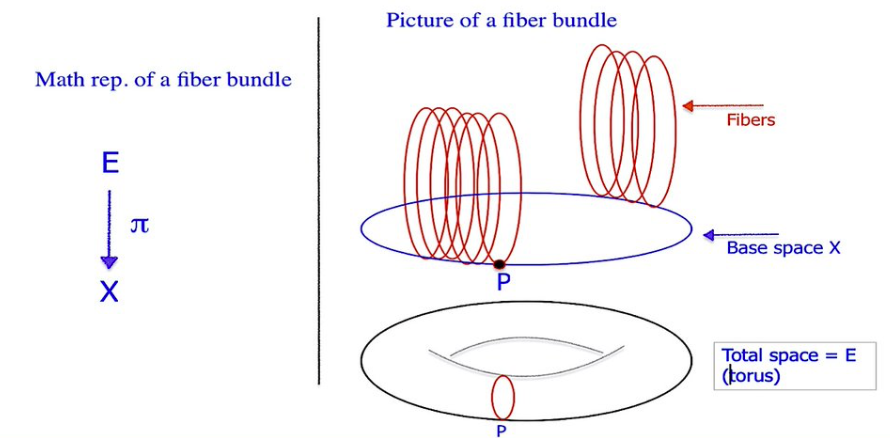
\includegraphics[width=0.85\linewidth]{Image5.png}
\end{figure}

\end{frame}


\begin{frame}{Example: Annulus as a Bundle}
Take real numbers \(0 \le r_0 < r_1\). Define
\begin{align*}
E = \{ (x,y) \in \mathbb{R}^2 \mid r_0 \le x^2 + y^2 \le r_1 \}, \quad
M = [r_0, r_1],
\end{align*}
and the projection
\begin{align*}
\pi: E \to M,\; \pi(x,y) = \sqrt{x^2 + y^2}.
\end{align*}

Then \((E, \pi, M)\) is a bundle. The fiber over \(r\in [r_0,r_1]\) is
\begin{align*}
E_r = \{ (x,y) \mid x^2 + y^2 = r^2 \},
\end{align*}
i.e.\ the circle of radius \(r\). The total space is an annulus. This is an example of an \(I\)-bundle (interval-bundle) over a circle base.

A section would pick one point on each circle: e.g.\ define
\begin{align*}
s(r) = (r, 0),
\end{align*}
then \(\pi(s(r)) = r\).
\end{frame}

\begin{frame}{Visualization}
    \begin{center}
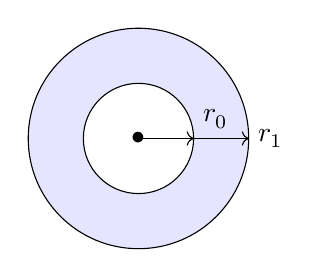
\begin{tikzpicture}[scale=0.7]
\draw[fill=blue!10] (0,0) circle (2);
\draw[fill=white] (0,0) circle (1);
\draw (0,0) node {$\bullet$};
\draw[->] (0,0)--(2,0) node[right] {$r_1$};
\draw[->] (0,0)--(1,0) node[above right] {$r_0$};
\end{tikzpicture}
\end{center}
\end{frame}

\begin{frame}{Proposition}
\vspace{-0.3cm}
\begin{block}{}
A function \( f : X \to Y \) is \textbf{bijective} if and only if it has a \textbf{two–sided inverse}; that is,
\[
f \text{ is bijective } \iff \exists\, g : Y \to X \text{ such that }
g \circ f = \mathrm{id}_X \text{ and } f \circ g = \mathrm{id}_Y.
\]
\end{block}

\textbf{Proof}
\textbf{($\Rightarrow$)}
Assume \(f\) is bijective.
Then \(f\) is injective and surjective.

\emph{Existence of inverse function:}
For each \(y \in Y\), surjectivity ensures the existence of at least one \(x \in X\) such that \(f(x)=y\).
Injectivity guarantees that this \(x\) is unique.
Hence, we can define a well–defined function \(g : Y \to X\) by assigning \(g(y)=x\), where \(f(x)=y.\)

Now, for all \(x \in X\):
\[
(g \circ f)(x) = g(f(x)) = x,
\]
and for all \(y \in Y\):
\end{frame}

\begin{frame}{Proof}
\[
(f \circ g)(y) = f(g(y)) = y.
\]
Thus \(g\circ f = \mathrm{id}_X\) and \(f\circ g = \mathrm{id}_Y\); \(g\) is a two–sided inverse of \(f.\)

\medskip
\textbf{($\Leftarrow$)}
Conversely, suppose there exists \(g : Y \to X\) such that
\[
g \circ f = \mathrm{id}_X, \quad f \circ g = \mathrm{id}_Y.
\]
\emph{Injectivity:}
If \(f(x_1)=f(x_2)\), apply \(g\) to both sides:
\[
g(f(x_1)) = g(f(x_2)) \Rightarrow \mathrm{id}_X(x_1)=\mathrm{id}_X(x_2) \Rightarrow x_1=x_2.
\]
Hence \(f\) is injective.

\end{frame}

\begin{frame}{Proof}

\emph{Surjectivity:}
For any \(y \in Y\), set \(x=g(y)\). Then
\[
f(x)=f(g(y))=(f\circ g)(y)=\mathrm{id}_Y(y)=y.
\]
Therefore every \(y\in Y\) has a preimage, so \(f\) is surjective.

Since \(f\) is both injective and surjective, \(f\) is bijective. \(\square\)

\end{frame}


\begin{frame}{Notes}
\begin{itemize}
    \item In the bundle context, a section gives a right inverse of \(\pi\).
    \item If \(\pi\) also had a left inverse, that would force \(\pi\) to be injective, which bundle projections typically are not (because fibers often contain multiple points).
    \item Thus for a general bundle, \(\pi\) is surjective but not injective, so it has sections, but no inverse redefining \(\pi\) as bijection.
\end{itemize}

\end{frame}

\begin{frame}{Summary and Roadmap}
\begin{itemize}
  \item We have defined standard sets (\(\mathbb{N},\mathbb{Z},\mathbb{Q},\mathbb{R}\)) and positive subsets.
  \item We introduced predicate/set-builder notation, Cartesian products, and matrices.
  \item Reviewed logical connectives and quantifiers; gave continuity, uniform continuity.
  \item Covered set operations (union, intersection, difference, power set) and the Cartesian product.
  \item Defined functions, composition, identity, and equality of functions.
  \item Introduced injectivity, surjectivity, bijectivity, and the connection to inverses (left, right).
  \item Introduced bundles, projections, fibers, and sections, with a concrete annulus example.
\end{itemize}

\end{frame}

%==============================
\section{Exercises / Homework}
%==============================

\begin{frame}{Homework}
Prove or disprove:
\begin{enumerate}
    \item $f$ injective $\iff$ $f$ has a left inverse.
    \item $f$ has right inverse $\implies$ $f$ surjective.
    \item $f$ surjective $\implies$ $f$ has right inverse.
    \item $f$ bijective $\iff$ $f$ invertible.
    \item Decomposition into fibers is indeed a disjoint union: $E = \bigsqcup_{x\in M} E_x$ is a disjoint decomposition into fibers.\\
    If \(\pi: E \to M\) is a surjection, then \(E = \bigsqcup_{x\in M} \pi^{-1}(x)\) and for \(x \neq y\), \(\pi^{-1}(x) \cap \pi^{-1}(y) = \emptyset.\)
\end{enumerate}
\end{frame}

\begin{frame}{Thanks}
  \cmcendframe
\end{frame}

\end{document}
